%%%  04.10.2013  %%%
%%%  VO 02
\section{Trees and Forests}

\begin{definition}
\index{forest}
A \dt{forest} is an undirected acyclic graph.
\end{definition}

\begin{definition}
\index{tree}
A \dt{tree} is a connected forest.
\end{definition}

\begin{definition}
\index{tree!rooted}
\index{root}
A \dt{rooted tree} is a tree with one special node designated as the \dt{root}.
\end{definition}

\begin{definition}
\index{tree!plane}
A \dt{plane tree} is a tree embedded into the plane, i.\,e. the order of
children matters. Two trees may be isomorphic, but not equivalent when regarded
as plane trees.
\end{definition}

In Computer Science, trees are often plane and rooted, e.\,g.\ binary search trees.

\begin{definition}
\index{isomorphism}
Two graphs $G$ and $H$ are \dt{isomorphic} ($G \cong H$) if there is a function
\[ \varphi: V(G)\mapsto V(H)\quad\text{$\varphi$ bijective} \]
so that
\[ vw \in E(G) \iff \varphi(v)\varphi(w) \in E(H). \]
\end{definition}

\begin{definition}
\index{leaf}
A \dt{leaf} is a node with degree 1. 
\end{definition}

\textbf{Lemma.}
A non rooted tree $T$ has at least 2 leaves. \\
$|V(T)| \geq 2$

\textbf{Proof.} \TODO{add images} \\
\begin{compactitem}
	\item T of size 2
	\item T of at least 3 nodes, $|V(T)| \geq 3$
	\begin{compactitem}
		\item Case 1:\\
			$|V(T)| = k+1 \Rightarrow |V(T)| = k$ \\
			$\Rightarrow_{imp} T'$ has 2 leaves $\Rightarrow T$ has at least 2 leaves
		\item Case 2: \\
			first node is no leaf, $T'$ and $T''$ each have at least 2 leaves each

	\end{compactitem}
\end{compactitem}


\begin{definition}
\index{bridge}
A \dt{bridge} is an edge whose removal would increase the number of connected components.
\end{definition}


\textbf{Theorem.} The following statements are equivalent:
\begin{compactenum}[(1)]
  \item $T$ is a tree.
  \item $\forall v,w\in V(T)$ $\exists$ unique path from $v$ to $w$
  \item $T$ connected, $|V(T)|=|E(T)|+1$
  \item $T$ minimal connected (every edge is a bridge)
  \item $T$ maximal acyclic
\end{compactenum}
\null\par

\textbf{Proof of 1. $\implies$ 3.} \\
induction on $n = \alpha_0=|V(T)|$

\begin{tabular}{l l}
	$n = 1:$	& trivial, $\cdot$ \\
	$n \rightarrow n+1:$	& Choose leaf $v$ of $T$, $T' = T \backslash \{v\}$ \\
							 &	
	$\begin{array}{ll}
	|V(T')| = |E(T')| + 1 \\
		|V(T')+1 = |E(T')+1 +1 \\
		substitution	& |V(T)| = |V(T')| +1 \\
			& |E(T)| = |E(T')| +1 \\
		|V(T)| = |E(T)| + 1
	\end{array}$
\end{tabular}

\subsection*{Spanning Subgraphs}

\begin{definition}
\index{spanning forest}
\index{spanning tree}
Let $G=(V,E)$ be an undirected graph. $F$ is a \dt{spanning forest} of $G$ if and only if:
\begin{compactitem}
  \item $V(F) = V(G)$, $E(F)\subseteq E(G)$,
  \item $F$ is a forest, and
  \item $F$ has the same connected components as $G$.
\end{compactitem}
If $F$ is connected, we call it a \dt{spanning tree}.
\end{definition}

\textbf{Example introducing matrix-tree theorem}\\

% Graph G and all possible spanning trees
\begin{figure}[htb]
\centering
\subfigure
{
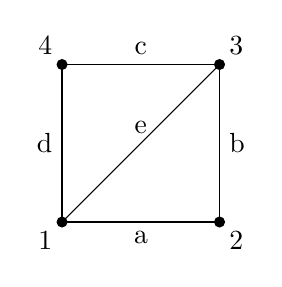
\begin{tikzpicture}[scale=2]

\node (n1) at (0,0) {};
\node (n2) at (1,0) {};
\node (n3) at (1,1) {};
\node (n4) at (0,1) {};

\draw (n1) node[anchor=north east] {$1$};
\draw (n2) node[anchor=north west] {$2$};
\draw (n3) node[anchor=south west] {$3$};
\draw (n4) node[anchor=south east] {$4$};

\foreach \i in {1,...,4}
{
	\fill (n\i) circle [radius=1pt];
};

\foreach \i/ \j/ \label/\position in {1/2/a/below, 2/3/b/right, 
					3/4/c/above, 4/1/d/left, 
					1/3/e/above}
{
	\path (n\i.center) edge node[\position] {\label} (n\j.center);
};
\end{tikzpicture}
}
\subfigure
{
	\begin{tabular}{cccc}
	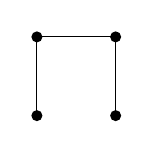
\begin{tikzpicture}

	\node (n1) at (0,0) {};
	\node (n2) at (1,0) {};
	\node (n3) at (1,1) {};
	\node (n4) at (0,1) {};

	\foreach \i in {1,...,4}
	{
		\fill (n\i) circle [radius=2pt];
	};

	\foreach \i / \j in {2/3, 3/4, 4/1}
	{
		\path (n\i.center) edge (n\j.center);
	};
	\end{tikzpicture}
	&
	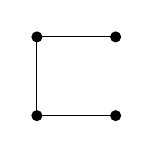
\begin{tikzpicture}

	\node (n1) at (0,0) {};
	\node (n2) at (1,0) {};
	\node (n3) at (1,1) {};
	\node (n4) at (0,1) {};

	\foreach \i in {1,...,4}
	{
		\fill (n\i) circle [radius=2pt];
	};

	\foreach \i / \j in {
	1/2, 
	%2/3, 
	3/4,
	4/1}
	{
		\path (n\i.center) edge (n\j.center);
	};
	\end{tikzpicture}
	&
	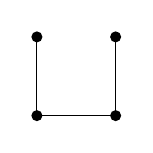
\begin{tikzpicture}

	\node (n1) at (0,0) {};
	\node (n2) at (1,0) {};
	\node (n3) at (1,1) {};
	\node (n4) at (0,1) {};

	\foreach \i in {1,...,4}
	{
		\fill (n\i) circle [radius=2pt];
	};

	\foreach \i / \j in {
	1/2, 
	2/3, 
	%3/4,
	4/1}
	{
		\path (n\i.center) edge (n\j.center);
	};
	\end{tikzpicture}
	&
	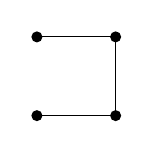
\begin{tikzpicture}

	\node (n1) at (0,0) {};
	\node (n2) at (1,0) {};
	\node (n3) at (1,1) {};
	\node (n4) at (0,1) {};

	\foreach \i in {1,...,4}
	{
		\fill (n\i) circle [radius=2pt];
	};

	\foreach \i / \j in {
	1/2, 
	2/3, 
	3/4}
	%4/1}
	{
		\path (n\i.center) edge (n\j.center);
	};
	\end{tikzpicture}
	\\
	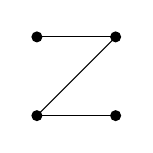
\begin{tikzpicture}

	\node (n1) at (0,0) {};
	\node (n2) at (1,0) {};
	\node (n3) at (1,1) {};
	\node (n4) at (0,1) {};

	\foreach \i in {1,...,4}
	{
		\fill (n\i) circle [radius=2pt];
	};
	\foreach \i / \j in {
	1/2, 
	%2/3, 
	3/4,
	%4/1,
	1/3}
	{
		\path (n\i.center) edge (n\j.center);
	};
	\end{tikzpicture}
	&
	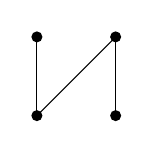
\begin{tikzpicture}

	\node (n1) at (0,0) {};
	\node (n2) at (1,0) {};
	\node (n3) at (1,1) {};
	\node (n4) at (0,1) {};

	\foreach \i in {1,...,4}
	{
		\fill (n\i) circle [radius=2pt];
	};
	\foreach \i / \j in {
	%1/2, 
	2/3, 
	%3/4,
	4/1,
	1/3}
	{
		\path (n\i.center) edge (n\j.center);
	};
	\end{tikzpicture}
	&
	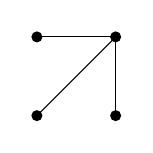
\begin{tikzpicture}

	\node (n1) at (0,0) {};
	\node (n2) at (1,0) {};
	\node (n3) at (1,1) {};
	\node (n4) at (0,1) {};

	\foreach \i in {1,...,4}
	{
		\fill (n\i) circle [radius=2pt];
	};
	\foreach \i / \j in {
	%1/2, 
	2/3, 
	3/4,
	%4/1,
	1/3}
	{
		\path (n\i.center) edge (n\j.center);
	};
	\end{tikzpicture}
	&
	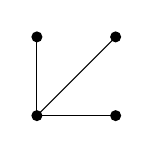
\begin{tikzpicture}

	\node (n1) at (0,0) {};
	\node (n2) at (1,0) {};
	\node (n3) at (1,1) {};
	\node (n4) at (0,1) {};

	\foreach \i in {1,...,4}
	{
		\fill (n\i) circle [radius=2pt];
	};
	\foreach \i / \j in {
	1/2, 
	%2/3, 
	%3/4,
	4/1,
	1/3}
	{
		\path (n\i.center) edge (n\j.center);
	};
	\end{tikzpicture}

	\end{tabular}
}
\caption{Graph $G$ and all its spanning trees}
\end{figure}





\begin{equation*}
\begin{array}{ll}
	\tilde A = \begin{pmatrix}
		0 & a & d & e \\
		a & 0 & 0 & b \\
		d & 0 & 0 & c \\
		e & b & c & 0 
	\end{pmatrix}
	&
	\tilde D = \begin{pmatrix}
		a+d+e \\
		& a+b \\
		& & c+d \\
		& & & b+c+e \\
	\end{pmatrix}
\end{array} 
\end{equation*}
\begin{equation*}
	\tilde D - \tilde A = \begin{pmatrix}
		\tikzmark{topA}a+\tikzmark{topA2}d+e & -a & -d & -\tikzmark{topB}e \\
		 -a & a+b & 0 & -b \\
		-d & 0 & c+d & -c \\
		-\tikzmark{botA}e & -b & -c & b+c+e \\
	\end{pmatrix}
\end{equation*}
\DrawLineHorizontal[red, thick, opacity=0.5]{topA}{topB}
\DrawLine[red, thick, opacity=0.5]{topA2}{botA}

\begin{equation*}
\begin{array}{ll}
\begin{vmatrix}
	a+b & 0 & -b \\
	0 & c+d & -c \\
	-b & -c & b+c+e
\end{vmatrix} 
& = (a+b)(c+d)(b+c+e)-b^2(c+d)-c^2(a+b) \\
& = bcd + abc+ abd +acd + ace + ade + bce + bde \\
& \text{every term represents a spanning tree}
\end{array}
\end{equation*}

if we set $a=b=c=d=1$ then

\begin{itemize}
	\item $\tilde A \rightarrow A$
	\item $\tilde D \rightarrow D = 
		\begin{pmatrix}3 \\ & 2 \\ & & 2 \\ & & & 3 \\ \end{pmatrix}$
	\item $det(D-A) = 8$
\end{itemize}

\textbf{Theorem (Kirchhoff's Matrix-Tree Theorem).}
Let
\begin{align*}
G &&& \text{undirected connected graph,} \\
A &&& \text{adjacency matrix,} \\
diag(d(v_1),\ldots,d(v_n)) = D &&& \text{degree matrix,} \\
(D-A)' &&& \text{$D-A$ with one row and one column removed.}
\end{align*}
Then $|\det{(D-A)'}|$ is the number of spanning trees of $G$.

\textbf{Remark.} If $G$ is not connected, the number of spanning trees can be
found for each connected component. Multiply results to get the number
of possible combinations.


% Minimal or Maximal Spanning Tree
% sub problem
% Minimal or maximal Spanning Trees
\begin{figure}[htb]
\centering
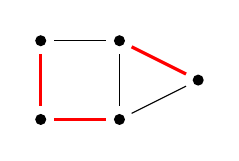
\begin{tikzpicture}[every node/.style = {circle}]

\node (a) at (0,0) {};
\node (b) at (1,0) {};
\node (c) at (2,0.5) {};
\node (d) at (1,1) {};
\node (e) at (0,1) {};
\foreach \node in {a,...,e}
{
	\fill (\node) circle [radius=2pt];
};

\draw[red,very thick] (a) -- (b);
\draw[red,very thick] (a) -- (e);
\draw[red,very thick] (c) -- (d);
%\draw (a) -- (b);
%\draw (a) -- (e);
\draw (b) -- (c);
\draw (b) -- (d);
%\draw (c) -- (d);
\draw (d) -- (e);
\end{tikzpicture}
\caption{Graph $G$ and its maximal spanning forest}
\end{figure}





% Proof: F_1, F_2 \sub E
% Observe:
% connecting the trees of a forest with edge e
\begin{figure}[htb]
\centering
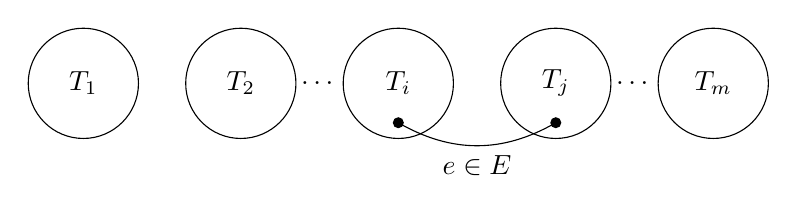
\begin{tikzpicture}
\node[] (T1) at (0,0) {$T_1$};
\node[] (T2) at (2,0) {$T_2$};
\node[] (T_dots1) at (3,0) {\ldots};
\node[] (Ti) at (4,0) {$T_i$};
\node[] (Tj) at (6,0) {$T_j$};
\node[] (T_dots2) at (7,0) {\ldots};
\node[] (Tm) at (8,0) {$T_m$};
\node[] (Ti_e) at (4,-0.5) {};
\node (Tj_e) at (6,-0.5) {};

\draw \foreach \n in {T1, T2, Ti,Tj,Tm}
{
	(\n) circle (0.7)
};

\fill (Ti_e) circle [radius=2pt];
\fill (Tj_e) circle [radius=2pt];

\path (Ti_e.center) edge [bend right] node[below] {$e \in E$} (Tj_e.center) ;

\end{tikzpicture}
\caption{Forest $F_2$ and its trees}
\end{figure}



\missingdate{2013-10-10}
\missingdate{2013-10-11}

